\documentclass[conference]{IEEEtran}
%% SECON 2013 addition:
\makeatletter
\def\ps@headings{%
\def\@oddhead{\mbox{}\scriptsize\rightmark \hfil \thepage}%
\def\@evenhead{\scriptsize\thepage \hfil \leftmark\mbox{}}%
\def\@oddfoot{}%
\def\@evenfoot{}}
\makeatother
\pagestyle{headings} 

\ifCLASSINFOpdf
  % \usepackage[pdftex]{graphicx}
  % declare the path(s) where your graphic files are
  % \graphicspath{{../pdf/}{../jpeg/}}
  % and their extensions so you won't have to specify these with
  % every instance of \includegraphics
  % \DeclareGraphicsExtensions{.pdf,.jpeg,.png}
\else
  % or other class option (dvipsone, dvipdf, if not using dvips). graphicx
  % will default to the driver specified in the system graphics.cfg if no
  % driver is specified.
  % \usepackage[dvips]{graphicx}
  % declare the path(s) where your graphic files are
  % \graphicspath{{../eps/}}
  % and their extensions so you won't have to specify these with
  % every instance of \includegraphics
  % \DeclareGraphicsExtensions{.eps}
\fi
% *** MATH PACKAGES ***
%
\usepackage[cmex10]{amsmath}
\usepackage{amsfonts}
\usepackage{graphicx, epsfig}
\usepackage{color}
\usepackage{subfigure}
\usepackage{xspace}
\usepackage{algorithm}
\usepackage{algpseudocode}
\usepackage{breqn}
\usepackage{cite}

\renewcommand{\thealgorithm}{}
\algnewcommand{\LineComment}[1]{\State \(\triangleright\) #1}
% A popular package from the American Mathematical Society that provides
% many useful and powerful commands for dealing with mathematics. If using
% it, be sure to load this package with the cmex10 option to ensure that
% only type 1 fonts will utilized at all point sizes. Without this option,
% it is possible that some math symbols, particularly those within
% footnotes, will be rendered in bitmap form which will result in a
% document that can not be IEEE Xplore compliant!
%
%\usepackage{array}
%\usepackage{mdwmath}
%\usepackage{mdwtab}
%\usepackage{eqparbox}
%\usepackage[tight,footnotesize]{subfigure}
%\usepackage[caption=false]{caption}
%\usepackage[font=footnotesize]{subfig}
%\usepackage[caption=false,font=footnotesize]{subfig}
%
%\usepackage{fixltx2e}

%\usepackage{stfloats}

%\usepackage{url}

% correct bad hyphenation here
\hyphenation{net-works}

\DeclareMathOperator*{\E}{\mathbb{E}}

\begin{document}
%
% paper title
% can use linebreaks \\ within to get better formatting as desired
\title{QoI Symptotics}

% author names and affiliations
% use a multiple column layout for up to three different
% affiliations

%\author{\IEEEauthorblockN{Scott Rager}
%\IEEEauthorblockA{Department of Computer Science and Engineering\\
%Pennsylvania State University\\
%University Park, PA 16802\\
%Email: rager@psu.edu}}

%\author{\IEEEauthorblockN{Scott Rager, Ertugrul Ciftcioglu, Thomas La Porta}
%\IEEEauthorblockA{Department of Computer Science\\
%and Engineering\\
%Pennsylvania State University\\
%University Park, PA 16802\\
%Email: rager@psu.edu, enc118@psu.edu, tlp@cse.psu.edu}
%\and
%\IEEEauthorblockN{Alice Leung, William Dron}
%\IEEEauthorblockA{Raytheon BBN Technologies\\
%Cambridge, MA 02138\\
%Email: aleung@bbn.com, wdron@bbn.com}
%\and
%\IEEEauthorblockN{John Hancock}
%\IEEEauthorblockA{Artistech\\
%City, State Zip Code\\
%Email: johnh@artistech.com}
%}

%\author{%
%  \IEEEauthorblockN{Scott T. Rager\IEEEauthorrefmark{1} \quad Ertugrul N. Ciftcioglu\IEEEauthorrefmark{1} \quad
%    \quad Thomas F. La Porta\IEEEauthorrefmark{1} \\ Alice Leung\IEEEauthorrefmark{2} \quad William Dron\IEEEauthorrefmark{2} \quad John Hancock\IEEEauthorrefmark{3} \\
%  }
%  \IEEEauthorblockA{
%  	\IEEEauthorrefmark{1}The Pennsylvania State University, University Park, PA 16802\\
%  \IEEEauthorrefmark{2}Raytheon BBN Technologies, Cambridge, MA 02138\\
%  \IEEEauthorrefmark{3}Artistech, Inc., Fairfax, VA 22030
%  }

%  Email:  str5004@psu.edu, enc118@psu.edu, tlp@cse.psu.edu, aleung@bbn.com, wdron@bbn.com, johnh@artistech.com
%\thanks{Research was sponsored by the U.S. Army Research Laboratory
%under the Network Science Collaborative Technology Alliance,
%Agreement Number W911NF-09-2-0053.} }


% for over three affiliations, or if they all won't fit within the width
% of the page, use this alternative format:
% 
%\author{\IEEEauthorblockN{Michael Shell\IEEEauthorrefmark{1},
%Homer Simpson\IEEEauthorrefmark{2},
%James Kirk\IEEEauthorrefmark{3}, 
%Montgomery Scott\IEEEauthorrefmark{3} and
%Eldon Tyrell\IEEEauthorrefmark{4}}
%\IEEEauthorblockA{\IEEEauthorrefmark{1}School of Electrical and Computer Engineering\\
%Georgia Institute of Technology,
%Atlanta, Georgia 30332--0250\\ Email: see http://www.michaelshell.org/contact.html}
%\IEEEauthorblockA{\IEEEauthorrefmark{2}Twentieth Century Fox, Springfield, USA\\
%Email: homer@thesimpsons.com}
%\IEEEauthorblockA{\IEEEauthorrefmark{3}Starfleet Academy, San Francisco, California 96678-2391\\
%Telephone: (800) 555--1212, Fax: (888) 555--1212}
%\IEEEauthorblockA{\IEEEauthorrefmark{4}Tyrell Inc., 123 Replicant Street, Los Angeles, California 90210--4321}}




% use for special paper notices
%\IEEEspecialpapernotice{(Invited Paper)}




% make the title area
\maketitle


%\begin{abstract}
%\boldmath
%The abstract goes here.
%\end{abstract}
% IEEEtran.cls defaults to using nonbold math in the Abstract.
% This preserves the distinction between vectors and scalars. However,
% if the conference you are submitting to favors bold math in the abstract,
% then you can use LaTeX's standard command \boldmath at the very start
% of the abstract to achieve this. Many IEEE journals/conferences frown on
% math in the abstract anyway.

% no keywords




% For peer review papers, you can put extra information on the cover
% page as needed:
% \ifCLASSOPTIONpeerreview
% \begin{center} \bfseries EDICS Category: 3-BBND \end{center}
% \fi
%
% For peerreview papers, this IEEEtran command inserts a page break and
% creates the second title. It will be ignored for other modes.
\IEEEpeerreviewmaketitle

%\begin{abstract}
%
%In many deployments of mobile ad hoc networks (MANETs), the primary goal is to collect and deliver data from many nodes to a designated operation center to support situation awareness and decision-making.  Additionally, this goal must be met while considering the limited resources, such as battery life, in the wireless nodes.  Traditional MANET protocols and research focus on providing protocols that are evaluated on performance criteria such as throughput and delay.  In this work, we extend this notion to include emphasis on the usefulness of data content along with traditional network state indicators such as current channel conditions to make cross-layer control decisions.  First we develop the notion of an information space created by generated data. Next, we formulate the problem of maximizing coverage over this information space while restricting individual node costs to remain within a given budget.  We then provide an algorithm that provides the solution to this problem.  Next we consider the related problem of finding the optimal long-term average coverage subject to average cost constraints and give its solution, which uses Lyapunov Optimization techniques.  For real world implementations, we also provide computationally feasible approximation algorithms for optimal solutions of both problems, including a novel technique that uses virtual queues for the average maximum coverage problem.  Finally, we provide simulation results of all proposed algorithms.  These results not only demonstrate the benefits of considering data content in scheduling, but also show the advantages from using the long-term average solution and the near-optimal performance of our greedy virtual queue approximation algorithm.
%
%\end{abstract}


\section{Introduction}
\label{sec:intro}

%area
Symptotic analysis is an emerging field of characterizing practical network scalability instead of the common asymptotic analysis.  Introduced in \cite{scalability_manets_theory_vs_practice}, symptotics is extremely useful for applications and network designers that are interested in determining the limits of a specific network implementation as well as how various factors affect these limits in terms of scalability.  For example, if one is designing an emergency mesh network to quickly install to replace destroyed infrastructure after a natural disaster, understanding the traffic limitations or what topology allows for the largest feasible network size is crucial to successful design.

%problem
%why not solved
While including the consideration of Quality of Information (QoI) into network control protocols or analysis is not novel, its limitations and effects on network scalability have not been considered before.  This consideration is extremely important, though, because in many recent fields of study, QoI is being used as the metric of a network's capabilities.  Increasingly, network nodes are becoming more capable of affecting QoI through data fusion, compression, selection, etc.  This work aims to begin understanding the connections between these actions and practical network scalability.

%insight
Specifically, in this work we consider the practical effects of real networks as protocol overhead, contention, rates in conjunction with QoI.  While adopting a general framework for QoI, we use timely, similarity-based image collection to provide motivation and concrete applications with results.  

%contribution
Our results first provide maximum sizes to which the networks can scale, given requested levels of QoI. The QoI depends on timeliness and one of two metrics considered: completeness or diversity.  These attributes are defined by the sum similarity of collected images resulting from Top-K queries for completeness, and sum dissimilarity of images collected using the greedy spanner algorithm. These definitions will be explained in more detail in Section \ref{sec:qoi_model}.  We observe that the network scalability considerably reduces with higher completeness and diversity requests, as well as with stringent timeliness requirements.  

Finally, we identify the trade-off of a given QoI requirement resulting in both a minimum required network size to provide a required number of images and the maximum feasible network size able to support that amount of necessary traffic.  We identify the region of QoI requests where the former does not exceed the latter, and, hence, the QoI request can be satisfied. 




\section{Symptotics Framework}
\label{sec:symptotics_bckgrnd}

Here, we provide an overview of the network scalability framework.




\section{QoI Examples}
\label{sec:qoi_examples}

The utility of data that is extracted from a sensor or military tactical network is often highly dependent on the context of the data with respect to aspects like the network's goals and the other data being collected from the rest of the network.  While this effect is often very qualitative by nature, we introduce metrics here that provide real examples of how QoI can be measured quantitatively.  These measures will then be used as examples in the QoI-aware network scalability in Section \ref{sec:qoi_scalability}.  

As an example scenario, we choose a mobile network in which nodes generate photographs that are to exchanged or collected at one or more data sinks.  This example covers surveillance missions of military tactical networks or civilian/social scenarios, one example of which could be smartphone users contributing to an image-sharing application.  

Qualities like lightness, contrast, and color are all inherent to a photograph, and many techniques have been studied to compare photographs.  We use one such technique called Color and Edge Directivity Descriptor (CEDD) \cite{2008cedd}.  Using the CEDD vector of each image, we can compare any two images.  To achieve a scalar representation of similarity, from comparing two vectors, we use \emph{Tanimoto similarity} \cite{tanimoto}, $T_s$.  Naturally, to describe the dissimilarity, or distance, of two photographs, then, we simply use $T_d = 1 - T_s$.

\subsection{Image Selection Algorithms}

With the Tanimoto similarities and distances between all of the images, a chosen algorithm can be applied to select images to provide a desired level of quality of information.  We present two such possibilities here along with examples and scenarios.

The first application of selecting images based on content occurs when a user would like to find more images that are similar to one already obtained.  For example, if a user observes a picture of an unknown suspicious person entering a building, but the person is not identifiable from that image, it would be useful to collect more images that are similar to that one with the possibility that another picture of the building from another user may have a better view of the person in question that can be used for identification or more context.  Called \emph{Top-k}, this algorithm choose the $k$ images with the smallest distance from the given image.  

The second application we introduce is called a \emph{spanner}, and it is based on an opposing scenario.  Instead of  choosing matching images, the goal of a spanner is to select the $k$ images that exhibit the most joint dissimilarity.  This algorithm would be useful in a surveillance mission or other setting in which a user would like to get a snapshot of all areas of which photographs were taken that is as complete as possible.  In order to choose images with the most dissimilarity, though, we must first define what that means.  While the dissimilarity between two images is determined by the Tanimoto distance, creating a measure of the distance between more than two images requires consideration.  

\subsection{QoI vs. Throughput}

With both the Top-k and Spanner algorithms, initial choices exhibit higher degrees of similarity and dissimilarity, respectively, that naturally decrease.  Therefore, if we establish a measure of overall QoI being obtained as $k$ is increased, we witness an effect of diminishing returns.  For the Top-k algorithm, we define \emph{Sum Similarity}, which is the sum of the Figures \ref{fig:spanCumDistReg} and \ref{fig:spanCumDist} show the diminishing returns of using similarity and dissimilarity metrics.

This effect is important also because it visually shows how Quality of Information differs from throughput.  As these graphs clearly show, transmission of successive images is not linear in terms of gained completeness.  Inversely, this relationship shows that obtaining a certain value of QoI or completeness may require a different number of images depending on the set available and their similarities.  Specifically, we can denote the number of images required to achieve a level of completeness, $S$, as $N(S)$.  This relationship will be useful later in determining feasible scalability.


If necessary, here, we could also include the toy examples of which pictures are actually selected from the top-k and spanner algorithms, showing that they are useful tools.




%Top-k Sum Similarity
%\begin{figure} 
%\begin{centering}
%    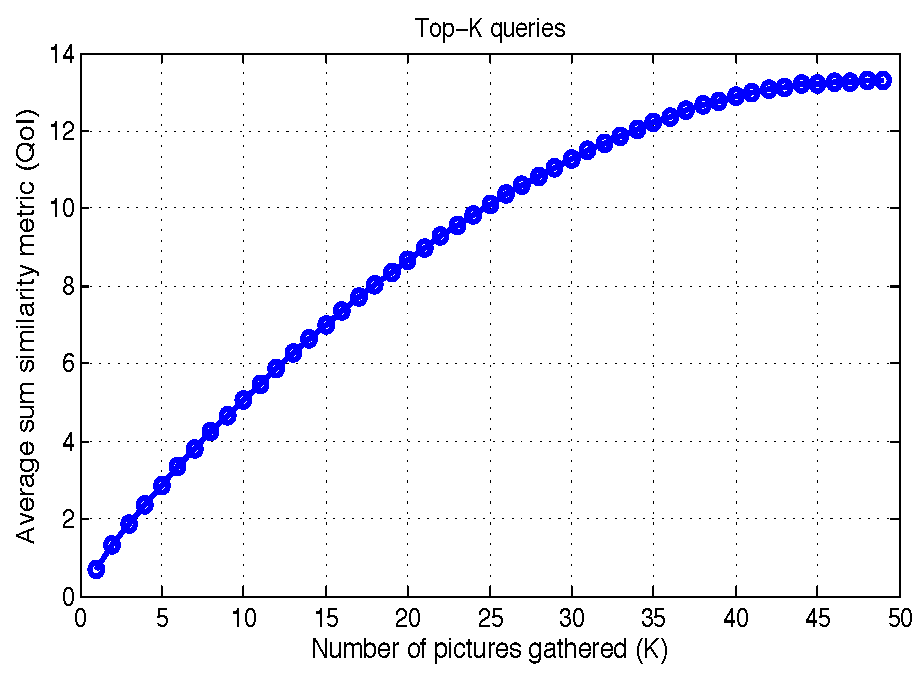
\includegraphics[scale=0.45]{figures/topkSumSimilarity.pdf}
%    \caption{Sum Similartiy for Top-k Results of Varying $k$}
%    \label{fig:spanAddDist}
%\end{centering}
%\end{figure}

%Spanner Cumulative Distance
\begin{figure} 
\begin{centering}
    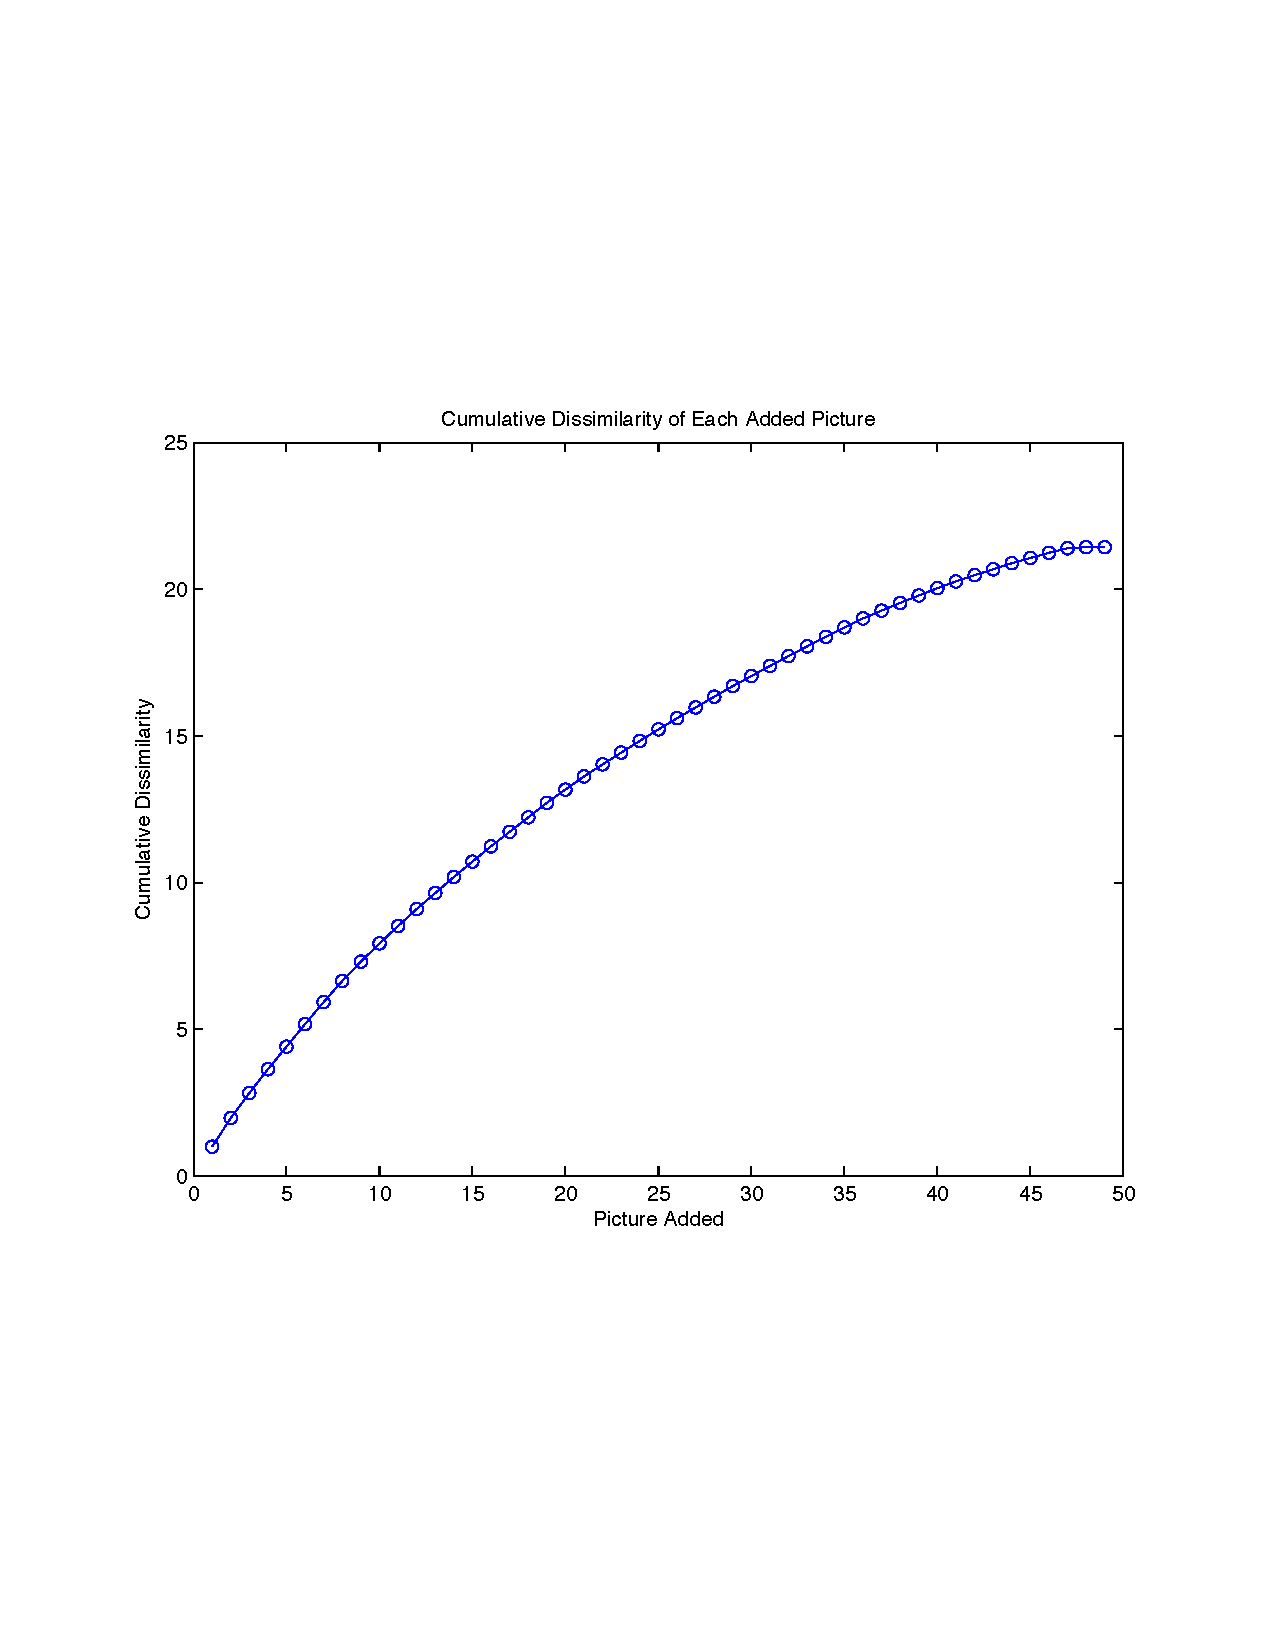
\includegraphics[scale=0.35]{figures/spannerCumulativeDist.pdf}
    \caption{Cumulative Distances for Spanners of Varying $k$ - Regular}
    \label{fig:spanCumDistReg}
\end{centering}
\end{figure}

%Spanner Cumulative Distance
\begin{figure} 
\begin{centering}
    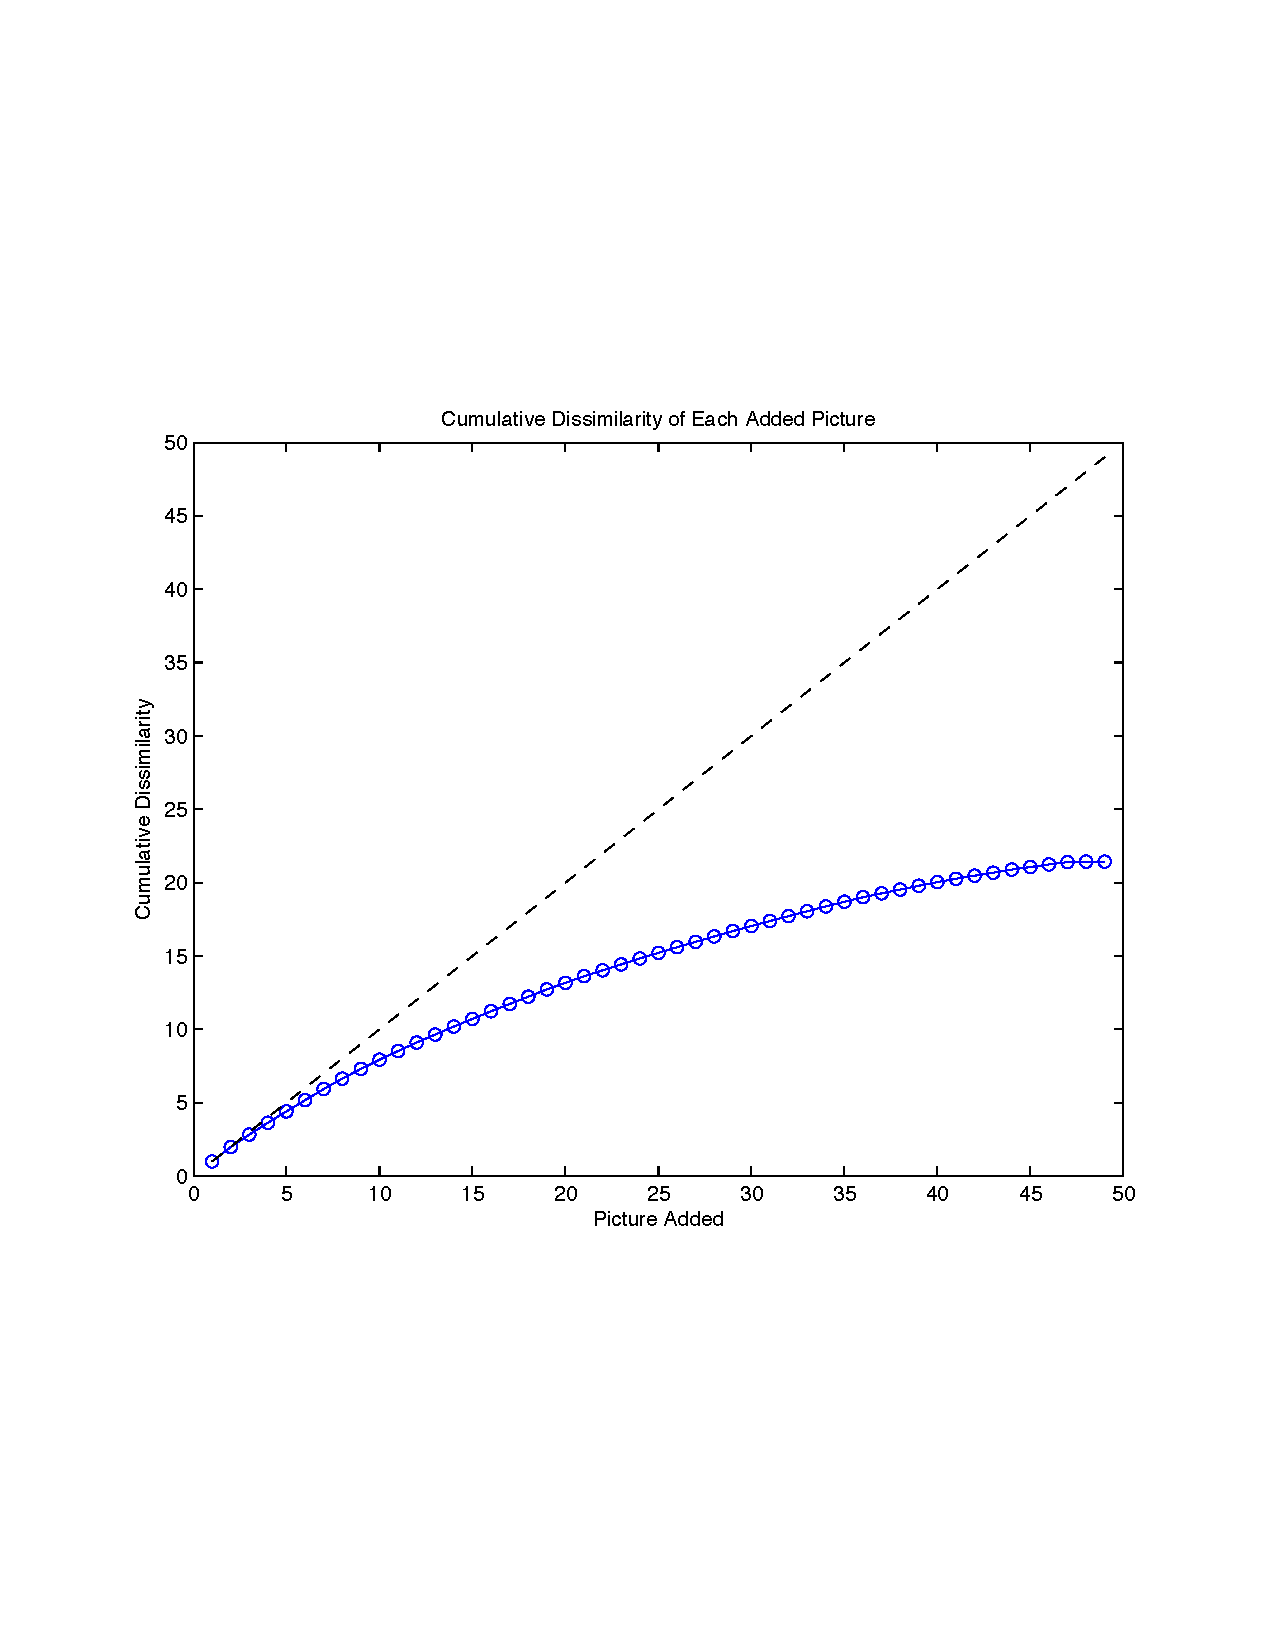
\includegraphics[scale=0.35]{figures/spannerCumulativeDistSquare.pdf}
    \caption{Cumulative Distances for Spanners of Varying $k$ - Square Axes}
    \label{fig:spanCumDist}
\end{centering}
\end{figure}





%As for how we were planning to relate a notion of QoI which is increasing with more images;
%The Top_K query seems readily expandable for different K-you give a target image and as you collect more images you add more "similarity metrics"(which reduces with distances), but the spanner had some issues:
%If normalized among all distances, the average distance among elements reduces with more elements.
%On the other hand, if we simply add pairwise distances, it overcounts too many combinations (n choose 2)
%So, the latest possibility I had in mind was to consider an additive metric such that each introduced picture brings increases the metric proportion to either the avg distance to existing elements, or minimum/maximum of all distances to the existing elements. 
%Given the definition of "spanner", which is "Spanner maximizes the minimum dissimilarity between all pairs", what  I had in mind was perhaps to consider an additive metric such that each introduced picture increases the metric proportion to the minimum of all distances to the existing elements. Or, since the whole set of selected pictures might change with different 
%K, probably the best metric is:
%
%For a spanner of K pictures: Total "quality/diversity metric" = \sum_{i=1 to K} min_{j in K-i} (distance_i, j)
%
%that is, we run the spanner, find K pictures. For each picture we have a minimum dissimilartity/distance to rest of the pictures. Than, we add these minimum dissimilarities over all pictures. 
%I think the case where the extra metric added is in proportion to the average distances should decrease for each new added picture, so we should have a increasing concave type function.

%the graph is generated as follows: 
%given a timeliness T and dissimilarity(D)/similarity(S) requirement, we find how many nodes the network can scale up to, say N, by the scalability analysis formulas.
%Then we look at how many images are required for attaining D/S, say K(this comes from the CEDD based MATLAB analysis). With the assumption that each node has one image, this essentially implies a lower bound on the required network size in terms of number of nodes to attain D/S.
%If N<K, the network cant actually scale large enough to provide the similarity/dissimilarity, so it is not "scalably feasible".
%so this graph is obtained as follows; for each T, identify the largest D/S such that N>=K still holds.

\section{QoI Scalability}
\label{sec:qoi_scalability}

\begin{figure}
\centering
    \subfigure[$TF = 2$, $CF = 3$, $DF = 1$]{
        \includegraphics[scale=0.28, clip=true, trim=5mm 0mm 5mm 0mm, valign=t]{delay_expl_fig_a.pdf}
        \label{fig:delay_expl_fig_3}
        }
    \subfigure[$TF = 2$, $CF = 3$, $DF = 2$]{
        \includegraphics[scale=0.28, valign=t]{delay_expl_fig_b.pdf}
        \label{fig:delay_expl_fig_4}
        }

   \caption{Example of line network using TDMA highlighting source of delays. (Node labels are TDMA slot assignments.)}
   \label{fig:both_delay_figures}
   \vspace{-5mm}
\end{figure}

Given the nonlinear returns of completeness and importance of timeliness outlined in the previous section, we contend that simply establishing the highest average supportable rate should not be the only goal of a QoI-aware network.  With this knowledge, we set the goal of determining the capacity of a network (and relatedly, the scalability achievable) with respect to {\em QoI requirements}, instead of the maximum throughput.  

\subsection{QoI Satisfiability Framework}
In order to establish the framework, we examine an arbitrary flow, $F_1$, in the network that has a QoI requirement of $\mathbf{q} = \{C, T\}$, where $C$ is the minimum required completeness metric of choice, such as sum similarity as explained above, and $T$ is the required timeliness.  This flow will have a data size requirement, which is given by a chosen QoI function $Q(C)$ like those discussed in Section \ref{sec:qoi_model}.  Using the example applications from \ref{sec:qoi_model}, for example, $Q(C)$ can return the number of images, $k_{req}$, required to achieve the requested completeness $C$ according to established relations like those in Section \ref{sec:qoi_model}.  Assuming each image has an average size of $I_S$, then we can also use $B$ to describe the total number of bits required by the flow, $B=k_{req}*I_S$.  To match realistic network implications, we assume this data will be transmitted in a series of packets with size $P_S$ bits each.  The number of packets per flow, then, is simply $P_N = \lceil B/P_S \rceil$.  We assume that each node in the network can transmit at $W$ bits per second when it is allocated media access.

Our goal is to establish the limits at which this arbitrary flow on average can no longer be completed with the QoI requirements satisfied.  We build and explain our model for achieving this goal by working through an example TDMA line network, a portion of which is shown in Figures \ref{fig:delay_expl_fig_3} and \ref{fig:delay_expl_fig_4} (We discuss addressing non-TDMA networks in Section \ref{sec:discussion}).  In this network, we assume a simple 3-slot TDMA scheme, which allows each node equal time access to the medium and removes any potential interference or hidden terminal issues.  Each node in the figure is labeled with its allocated slot.  For simplicity, we will assume that one slot is appropriately sized to transmit a single packet, i.e., $T_{slot} = P_S/W$ and that packets use static routes calculated beforehand such that the overhead is not a consideration here.

Now, two factors, $D_1$ and $D_2$, contribute to the total delay of completing $F_1$.  The first contributor, $D_1$, is the end to end delay incurred by sending the $B$ bits across the entire path.  To quantify this delay, we must consider several factors beyond just the available bandwidth and number of packets.  First, each node can only utilize its allotted channel time, creating a Channel Factor of $CF = N_{frame}/N_{i}$, where $N_{i}$ is the number of slots allocated to node $i$ and $N_{frame}$ is the total number of slots in each frame.  In this case, $N_{i} = 1, \forall i$ and $N_{frame} = 3$.  The second factor to consider for $D_1$ is the fraction of allocated slots that are utilized by the node to serve flows other than $F_1$ that are either originating in or being routed through nodes on the path of flow $F_1$.  We call the total number of flows competing at node $i$ the Traffic Factor, $TF_i$, of that node.  For any flow, the maximum contributor to delay is the node along the path with the maximum $TF_i$, which we will just call $TF$ here.  Incorporating these considerations into a calculation for $D_1$, we achieve the following expression


\begin{equation}
	D_1 = T_{slot} \cdot P_N \cdot CF \cdot TF
\end{equation}
%\begin{figure}
%\begin{centering}
%    \includegraphics[scale=0.33]{figures/delay_limit_expl/delay_expl_fig_a.pdf}
%    \caption{Example of line network using TDMA highlighting source of delays, $D_1$ and $D_2$.  Here, $TF = 2$, $CF = 3$, and $DF = 1$. }
%    \label{fig:delay_expl_fig_3}
%    \vspace{-3mm}
%\end{centering}
%\end{figure}

Figure \ref{fig:delay_expl_fig_3} depicts the delay of $D_1$ in a simple case of only two flows, $F_1$ and $F_2$, being present, in which case $TF = 2$.  In this example we use flows that consist of only $2$ ($F_{i-j}$ is packet $j$ in flow $i$) packets to portray the delay.  In most real applications, $P_N$ will be much larger, making $D_1$ a good approximation of this delay component.

%\begin{figure}
%\begin{centering}
%    \includegraphics[scale=0.35]{figures/delay_limit_expl/delay_expl_fig_b.pdf}
%    \caption{In the opposite direction, $DF = 2$. ($TF$ and $CF$ are unchanged here.)}
%    \label{fig:delay_expl_fig_4}
%\vspace{-5mm}
%\end{centering}
%\end{figure}

The second delay that exists is due to multi-hop propagation of packets.  This delay is simply the time for a single packet to traverse the path length.  Note that this delay is not necessarily just the path length multiplied by $T_{slot}$, because of possible queuing delays and/or ordering constraints.  We show here how ordering constraints impact this TDMA network.  A node cannot forward a packet from the flow until it receives that packet from the previous hop.  In our line network example, when the direction of the flow matches the nodes' schedule of slots $1-2-3-1-2-3$, as in Figure \ref{fig:delay_expl_fig_3}, each successive node receives a packet on the time slot before it is scheduled, resulting in no extra delay.  For a flow in the opposite direction, though, where nodes are scheduled $3-2-1-3-2-1$, as in Figure \ref{fig:delay_expl_fig_4}, the first slot $1$ is not utilized, because the first node scheduled in time slot $1$ has not yet received a packet in the flow.  Every other slot is wasted, on average, for the initialization of the flow, resulting in approximately twice the delay.  We will use a term that we call the \emph{Delay Factor}, or $DF$, to account for this effect where it exists.

The multi-hop propagation delay, then, is modeled by

\begin{equation}
	D_2 = T_{slot} \cdot DF \cdot (PL - 1)
\end{equation}
where $PL$ is the average path length.

We note several points about this delay factor.  First, in a loaded network, the nodes can and will serve other flows while awaiting the arrival of packets in this flow of focus.  That utilized bandwidth does not, however, preclude this $DF$ impact on delay for the flow of interest, $F_1$.  Any node cannot serve $F_1$ until a packet from that flow has been received.  Second, this delay is only accounted for once per flow because all other packets are pipelined.  All other packets' delay is captured by the end to end delay, $D_1$.  This effect is best illustrated by examining the difference between $D_2$ in Figures \ref{fig:delay_expl_fig_3} and \ref{fig:delay_expl_fig_4}.  Here, we see the multi-hop propagation requires twice the number of slots because every other slot is unused in $F_1$'s propagation.  
%Note that these unused slots may be used by the nodes to transmit packets from a different flow, so the bandwidth may be utilized, but since it cannot be used for flow $F_1$, the delay for this flow is still impacted by $DF$.

To calculate a $DF$ for an entire network, we can calculate a $DF$ for each possible sample path and find the average of these values.  For example, in the case of the line network with a $3$-slot schedule, $DF = 1$ in the direction for Figure \ref{fig:delay_expl_fig_3} and $DF = 2$ in the opposite direction shown in Figure \ref{fig:delay_expl_fig_4}, so the average $DF$ used to approximate average delay in the network is $DF_{line-avg}=1.5$.  

By combining the two components of delay, we can give a relation for a network that will successfully achieve an average flow's data and timeliness requirements:

\vspace{-2mm}
\begin{equation*}
	D_1 + D_2 \leq T 
\end{equation*}
\begin{equation*}
	T_{slot} \cdot P_N \cdot CF \cdot TF + T_{slot} \cdot DF \cdot (PL-1) \leq T
\end{equation*}

Recalling that the time of a slot is determined by the size of a packet, $P_S$, and available channel rate, $W$, in the relation $T_{slot} = P_S/W$, we can substitute to get
\begin{equation*}
	\frac{P_S}{W} \cdot P_N \cdot CF \cdot TF + \frac{P_S}{W} \cdot DF \cdot (PL-1) \leq T
\end{equation*}
Finally, substituting the total number of bits required for a flow $P_S \cdot P_N =  k_{req} \cdot I_S$ (where $k_{req}$ is given by a function of required QoI), and rearranging this inequality, we can obtain a cleaner view of each parameter's impact on network limits:

\vspace{-2mm}
\begin{equation}
	W \cdot T - k_{req} \cdot I_S \cdot CF \cdot TF - P_S \cdot DF \cdot (PL-1) \geq 0	
	\label{eq:general_scal}
\end{equation}

Every network will have its own set of parameters that can be substituted into this general formula, providing a tool to approximate limitations and sensitivity to changes in specific parameters.  To show this usefulness concretely, we provide derived values for a TDMA-based wireless network with several basic topologies.


\begin{figure*}[]
\centering
    \subfigure[Clique Network, $I_S = 9 MB$]{
        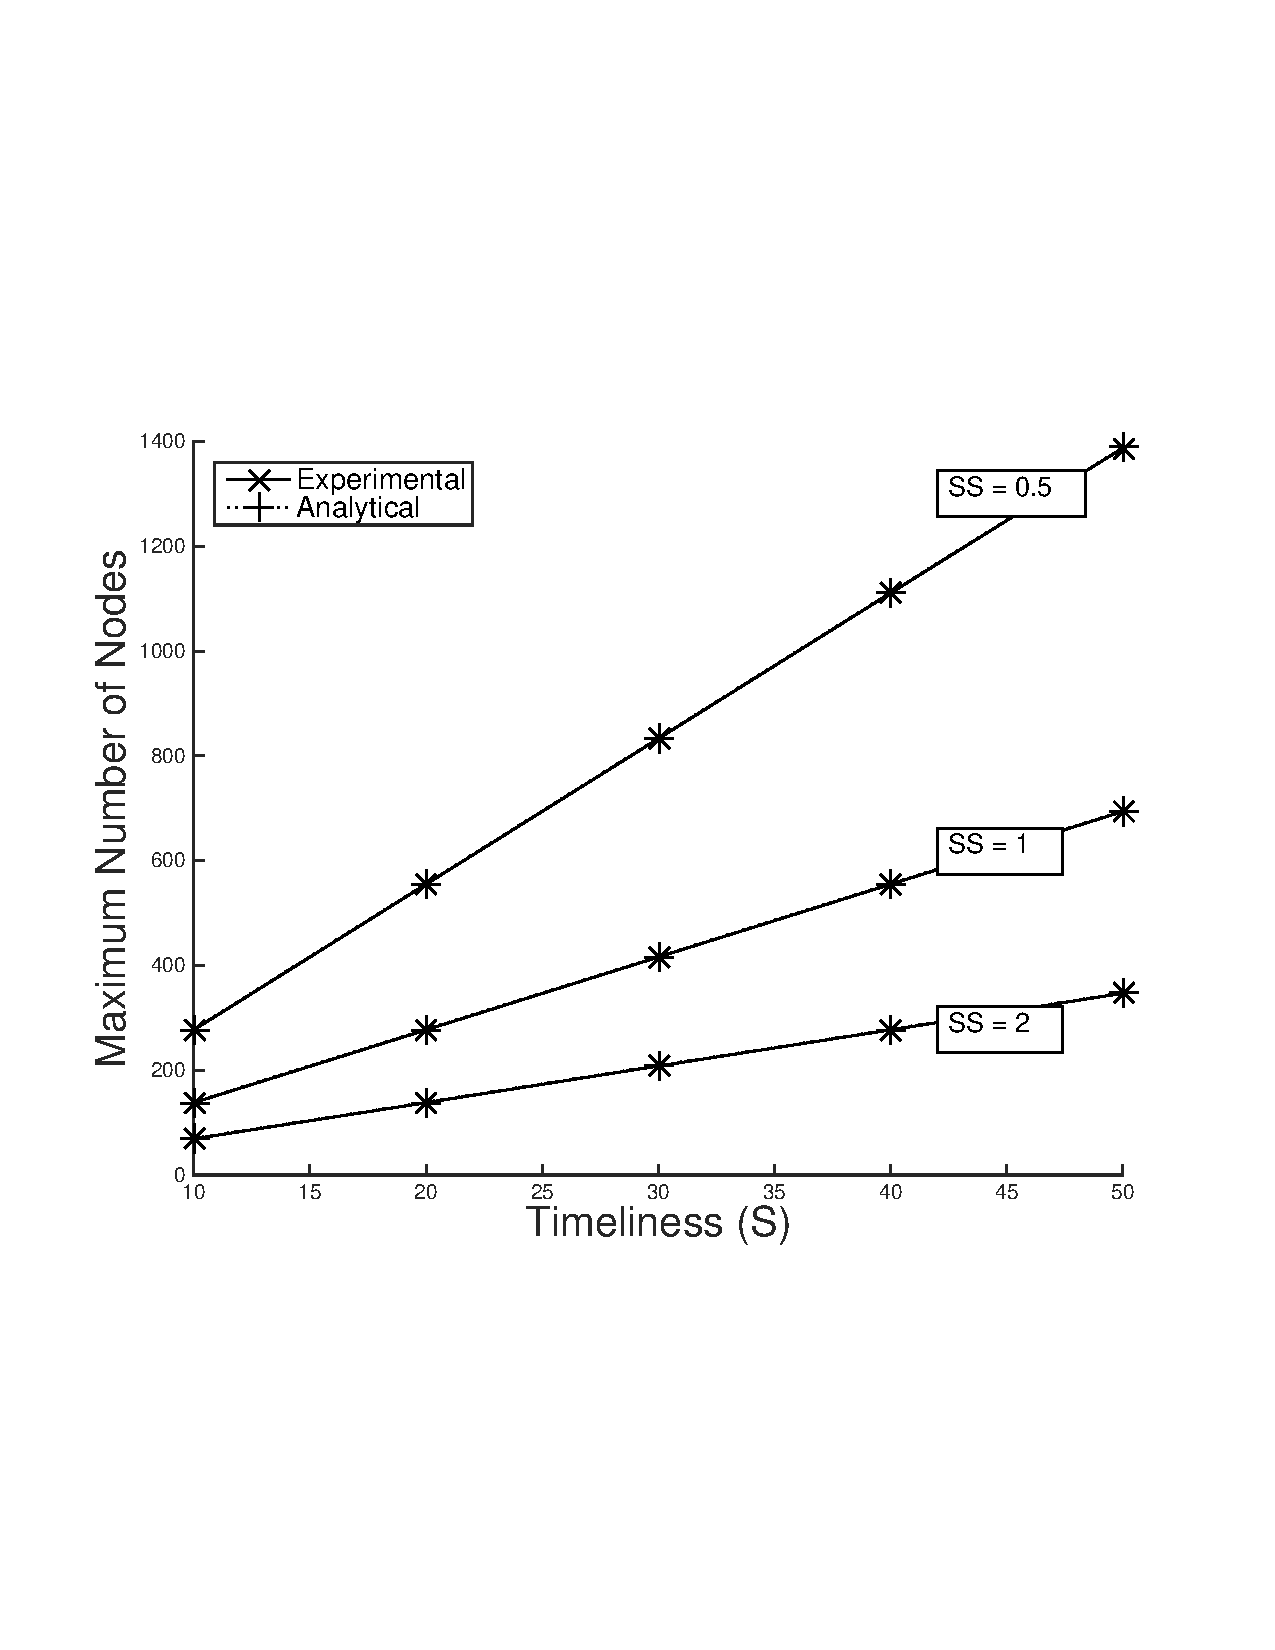
\includegraphics[scale=0.29, clip=true, trim=15mm 65mm 20mm 65mm]{clique_uni_2d.pdf}
        \label{fig:scal_vs_qoi_clique}
        }
    \subfigure[Line Network, $I_S = 12 MB$]{
        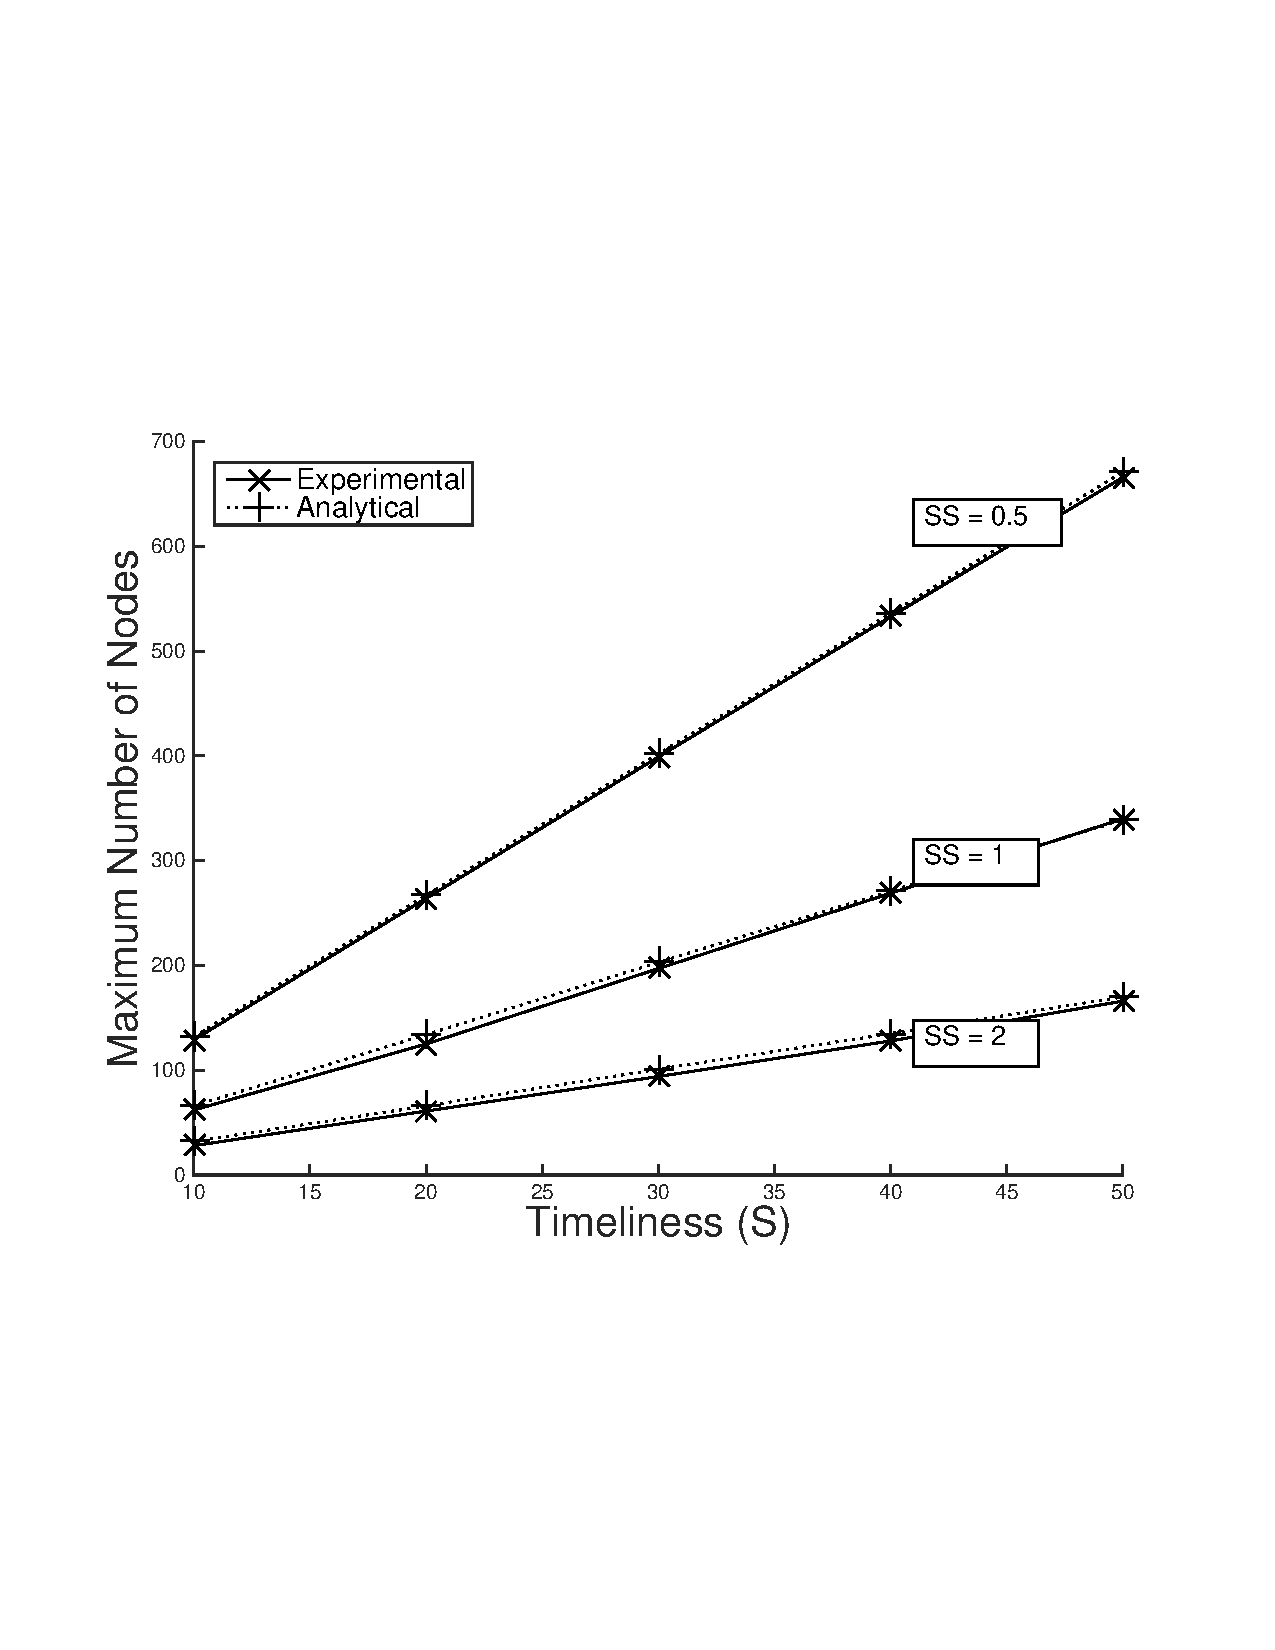
\includegraphics[scale=0.29, clip=true, trim=15mm 65mm 20mm 65mm]{line_uni_2d_mhop_2.pdf}
        \label{fig:scal_vs_qoi_line}
        }
    \subfigure[Grid Network, $I_S = 48 MB$]{
        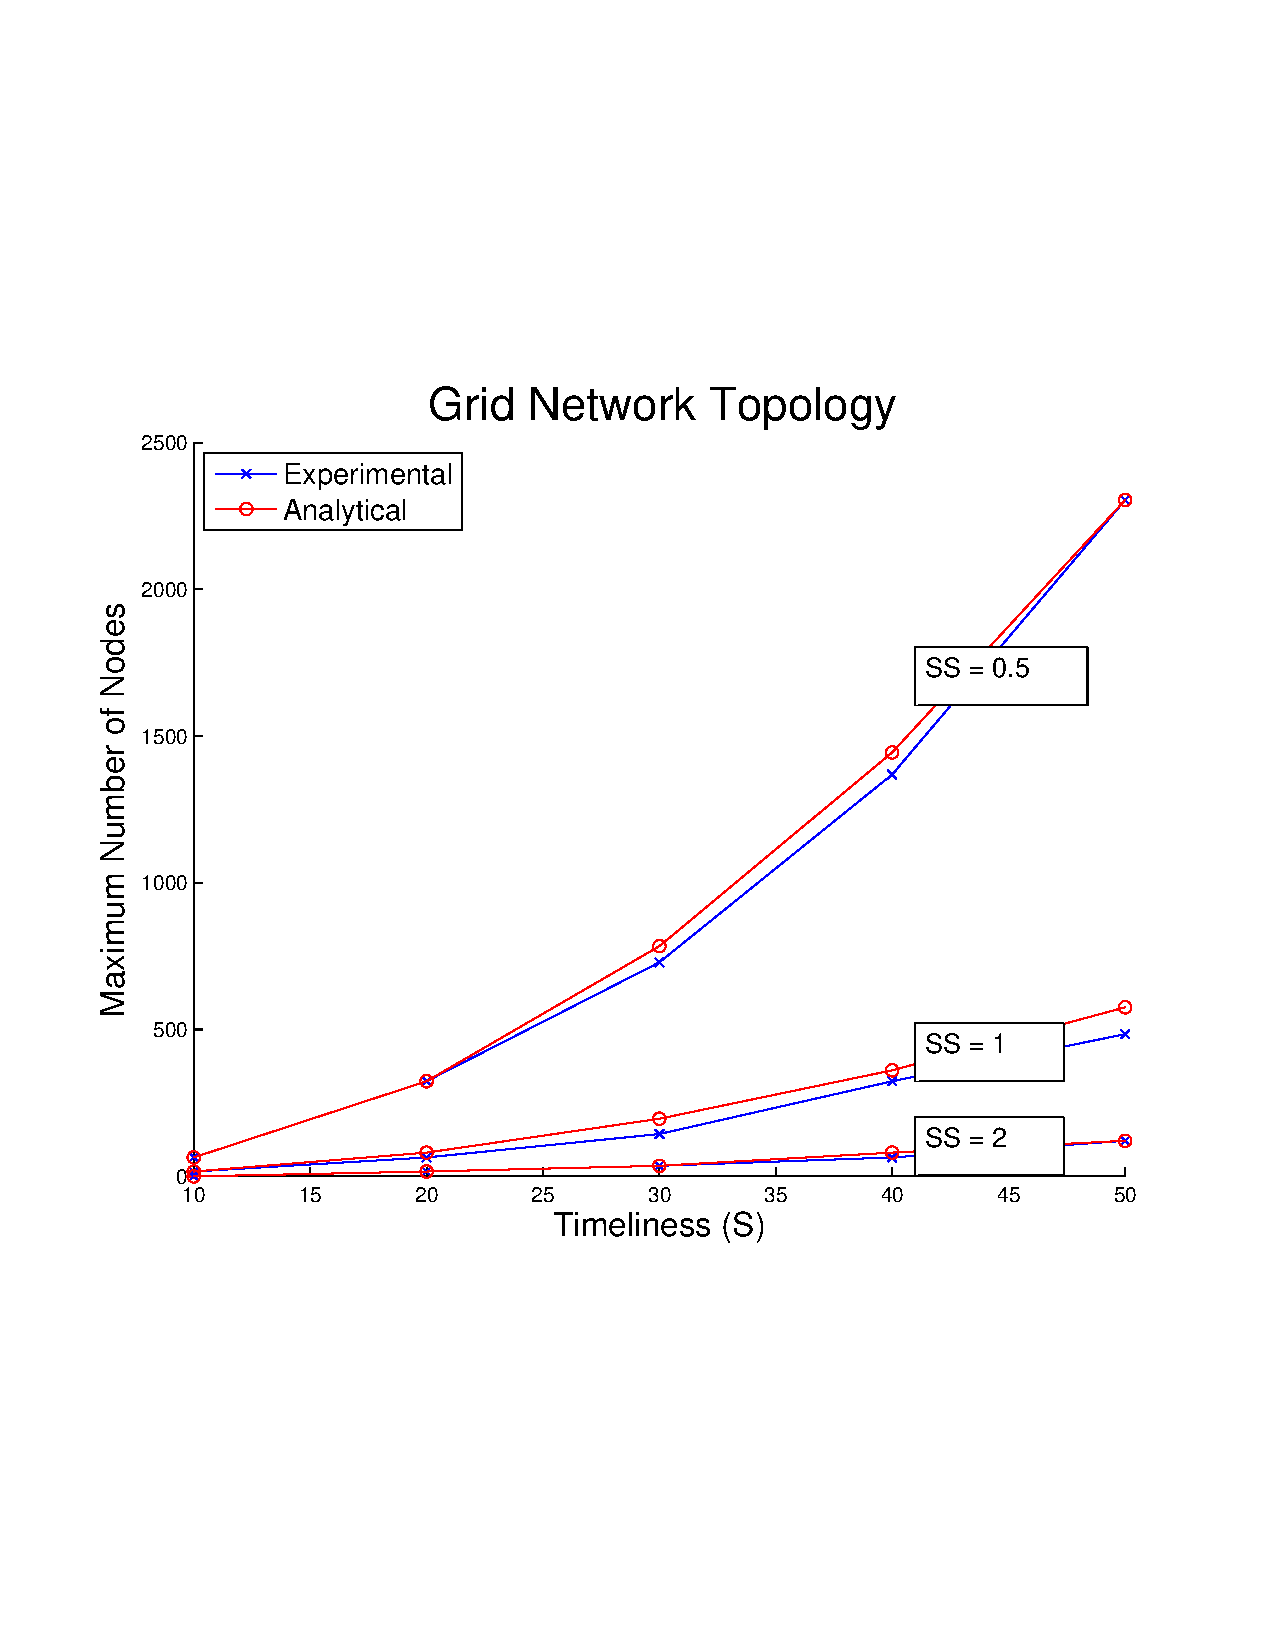
\includegraphics[scale=0.29, clip=true, trim=15mm 65mm 20mm 65mm]{grid_uni_2d_mhop_2.pdf}
        \label{fig:scal_vs_qoi_grid}
        }

   \caption{Empirical results match analytical results closely for all performed tests.  Results for each topology and a variety of sum similarity (SS) and timeliness requirements are provided.}
   \label{fig:scal_vs_qoi}

\vspace{-6mm}
\end{figure*}

\subsection{Example of Applying Framework}
\label{sec:example_apply_fw}

We illustrate the application of network signatures to the relationship in (\ref{eq:general_scal}) using an $N$-node TDMA network with three different topologies: clique, line, and grid, also known as a ``Manhattan grid.'' (Discussion of other network control protocols and topologies are addressed in Section \ref{sec:discussion}.)  We adopt a traffic model that uses Top-K queries as an example application.  We assume that all nodes have a set of collected images that are used to respond to Top-K queries.  Each node produces a query with a target image and target QoI, $\mathbf{q} = \{C, T\}$, describing the required completeness (here, we use sum similarity) and timeliness, and sends it to another node chosen at random.  The queried node will respond with the number of images, $k_{req}$, required to achieve the target sum similarity.  Values for $k_{req}$ are taken from the empirical relation in Figure \ref{fig:topkSumSim}\footnote{This application is not necessarily intended to model a known operational scenario, only a generic example to illustrate our model in a simple manner.}.  

\begin{table}[h]
\centering
\begin{tabular}{l|l|l|l|l|}
\cline{2-5}
                            					 & \textbf{CF}  					& \textbf{TF}   				& \textbf{DF}	& \textbf{PL} 			\\ \hline
\multicolumn{1}{|l|}{\textbf{Clique}} 	& N-1 							& 1                              		& 1  			& 1 					\\ \hline
\multicolumn{1}{|l|}{\textbf{Line}}   	& 3   							& $\frac{(N-1)^2}{2(N-2)}$ 	& 1.5 			& $\frac{N}{4}$			\\ \hline
\multicolumn{1}{|l|}{\textbf{Grid}}   	& 5   							& $\sqrt{N}$                       	&  2.5			& $\frac{2}{3} \sqrt{N}$   \\ \hline
\end{tabular}
\caption{CF, TF, DF, and PL values for example topologies}
\label{table:rf_ff_sf_values}
\vspace{-5mm}
\end{table}

Since our goal is to determine the point at which an average flow is no longer sustainable, we derive and use average values for $TF$, $CF$, $DF$, and $PL$ for the network.  In the case of $TF$, we use the value for the node with the largest expected $TF_i$ since flows that are routed through this node are expected to experience that largest delay and are likely to be the first that fail to meet their timeliness requirements.  Values for this example are shown in Table \ref{table:rf_ff_sf_values}, and a derivation of $TF$ for a grid network is included in Appendix \ref{sec:grid_tf_proof}.  Details about deriving the other values are explained in detail in \cite{symptotics_tech_report}.  The following equations can be used to determine QoI and network size limitations, which will be exemplified in the next two sections:

\vspace{3mm}
\noindent
Clique:
\begin{equation}
\label{eq:clique_gen}
	W \cdot T - I_S \cdot k_{req} \cdot (N-1) \geq 0
\end{equation}
Line:
\begin{equation}
\label{eq:line_gen}
	W \cdot T - 3 \cdot I_S \cdot k_{req} \cdot \frac{(N-1)^2}{N-2} - 1.5 \cdot P_S \cdot (\frac{N}{4}-1) \geq 0
\end{equation}
Grid:
\begin{equation}
\label{eq:grid_gen}
	W \cdot T - 5 \cdot I_S \cdot k_{req} \cdot \sqrt{N} - 2.5 \cdot P_S \cdot (\frac{2}{3}\sqrt{N} - 1) \geq 0
\end{equation}





\section{Results}
\label{sec:results}

In Figures \ref{fig:3dplots12} and \ref{fig:3dplots34}, we demonstrate network scalability as a function of QoI requirements for different traffic properties in a mesh setting.

\begin{figure}
\centering
    
    \subfigure[Unicast Traffic]{
        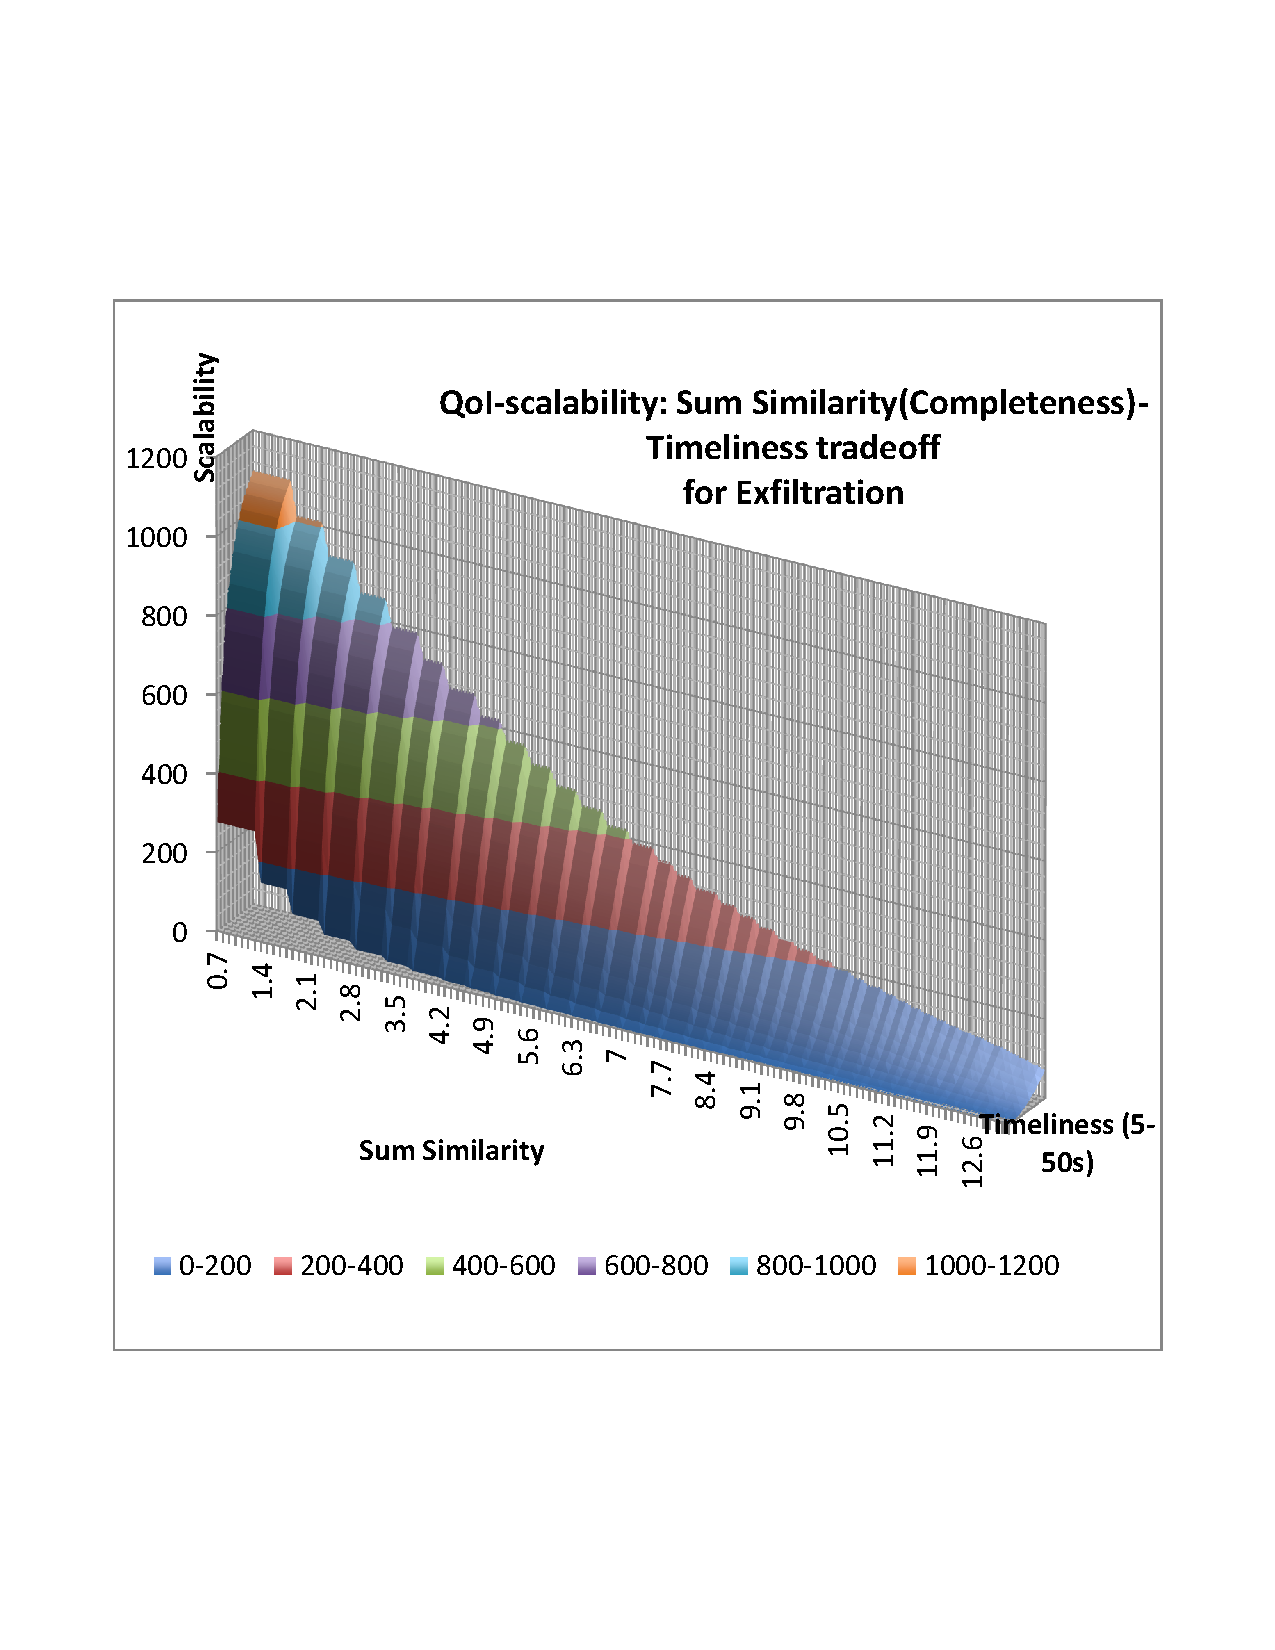
\includegraphics[scale=0.35]{figures/topk_uni.pdf}
        \label{fig:3dplot1}
        }

    \subfigure[Flooding]{
        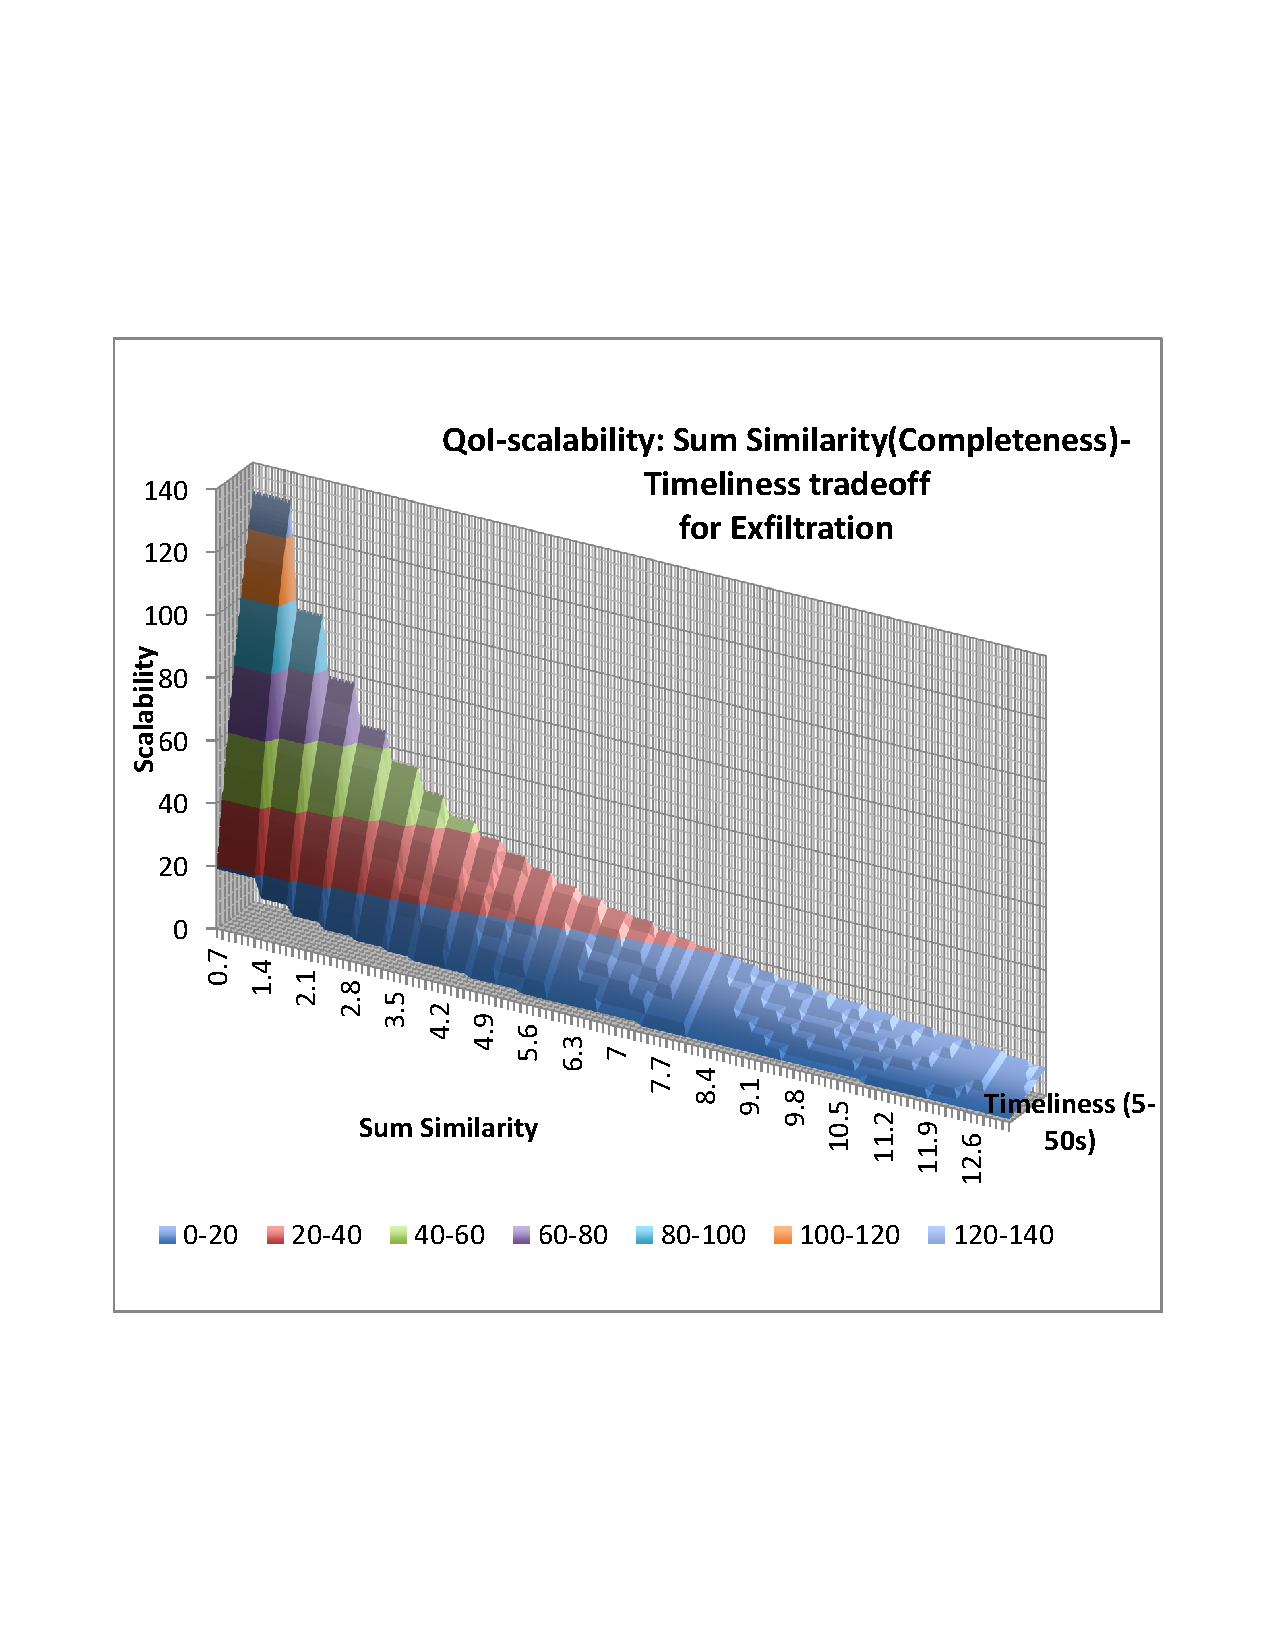
\includegraphics[scale=0.35]{figures/topk_fld.pdf}
        \label{fig:3dplot2}
        }

   \caption{Top-K:  Sum Similarity vs. Scalability vs. Timeliness}
   \label{fig:3dplots12}
\end{figure}


\begin{figure}
\centering
    \subfigure[Unicast Traffic]{
    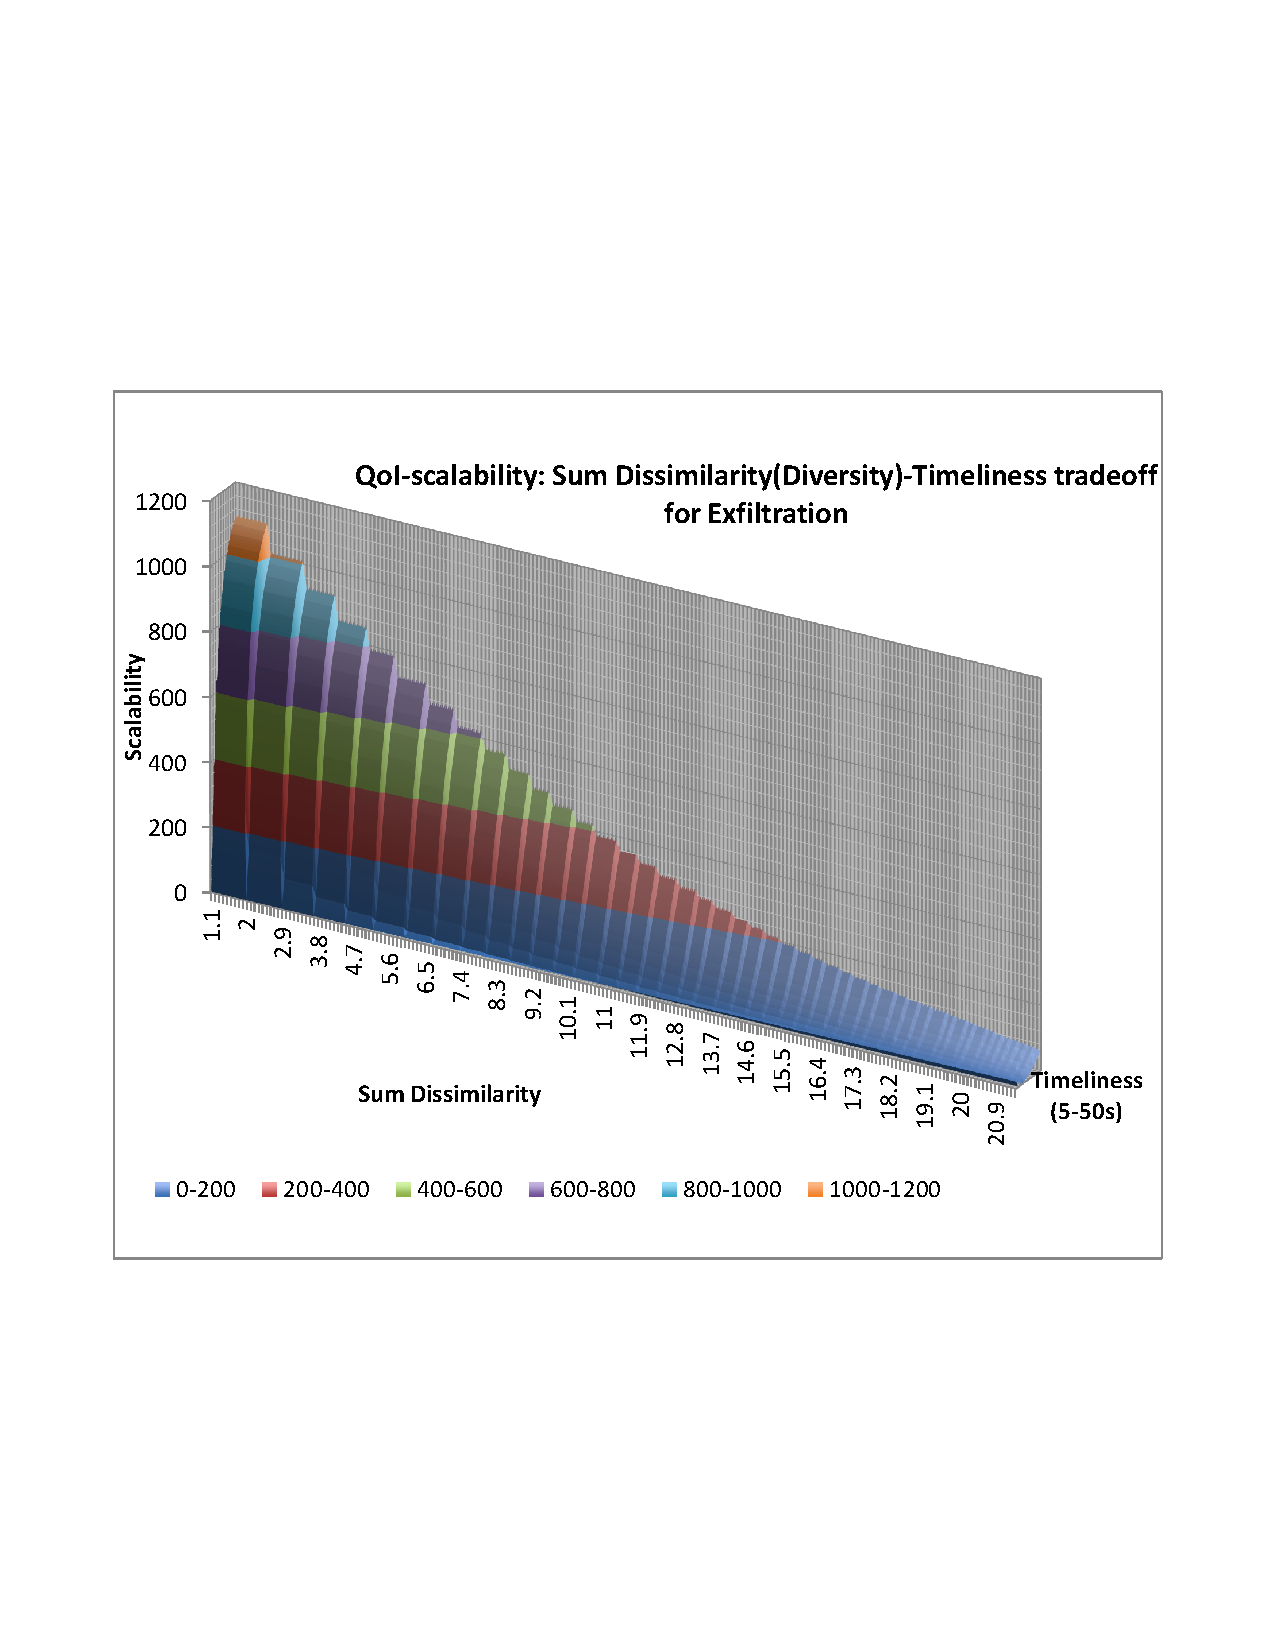
\includegraphics[scale=0.35]{figures/span_uni.pdf}
    \label{fig:3dplot3}
    }

    \subfigure[Flooding]{
    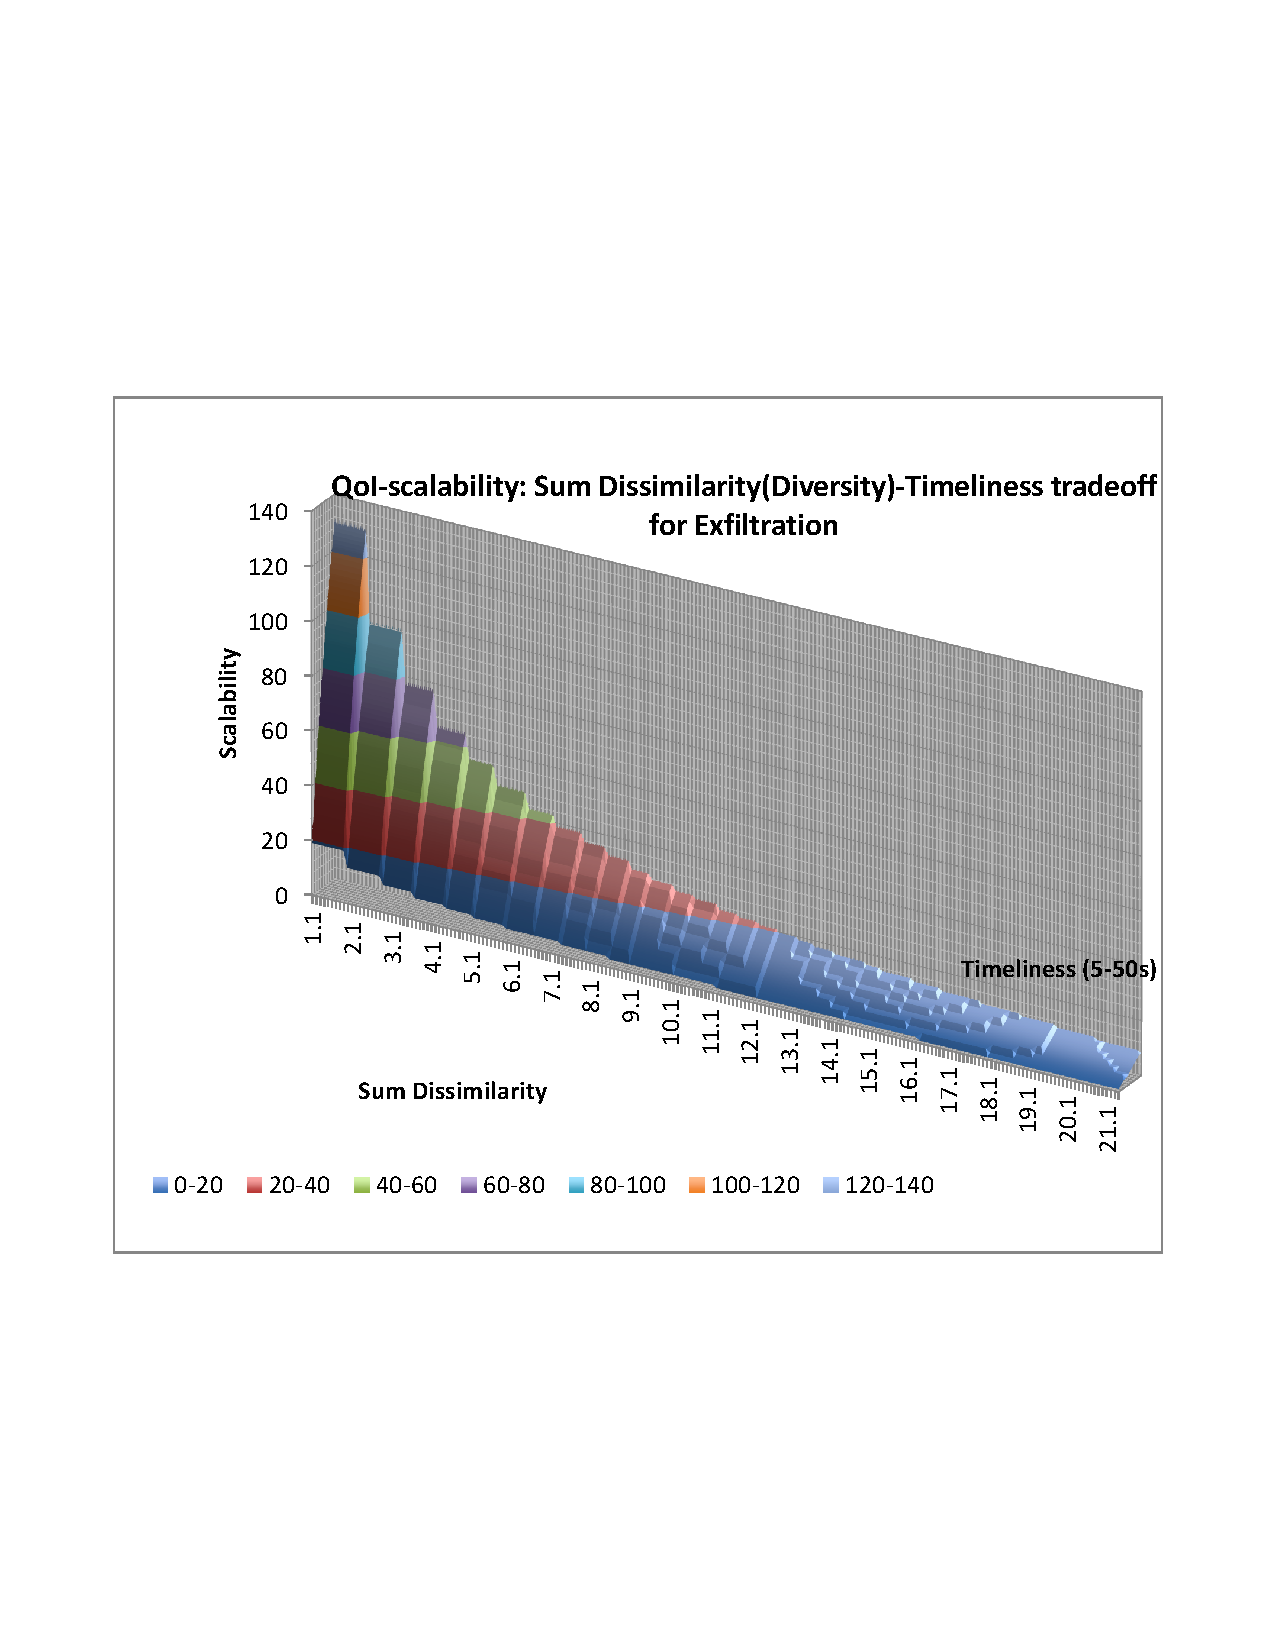
\includegraphics[scale=0.35]{figures/span_fld.pdf}
    \label{fig:3dplot4}
    }
   \caption{Spanner:  Sum Dissimilarity vs. Scalability vs. Timeliness}
      \label{fig:3dplots34}
\end{figure}

Clearly, there is a remarkable difference in the scalability depending upon
the QoI. 
The fact that QoI makes a difference is not surprising, but the {\em magnitude} of the
impact is surprising, along with the fact that there are some critical
thresholding points. Our preliminary work shows that
scalability analysis with QoI awareness has the potential to
open up new tradeoff points with
significant potential benefits in scalability. For instance, it can
potentially indicate when it makes sense to reduce QoI a bit and possibly
gain significantly in scalability (e.g. increasing timeliness constraints for small Sum Similarity/Dissimilarity values)
 %(e.g. from QoI=(10,5) to QoI=(10,10) in Figure    % These specific example points need fixed
%\ref{fig:scal-log}) 
and when such reductions will only give a marginal
increase in scalability
(e.g. increasing timeliness for high values of Sum Similarity/Dissimilarity).



\subsection{Scalably Feasible QoI Regions}
For the special case where each node possesses one image, we have observed the following dilemma. To achieve a certain level of desired QoI \text{q}, which can be defined as $(C,T)$ for Top-K queries and $(D,T)$ for spanner queries, the completeness/diversity attribute necessitates a number $K_{req}(q)$ images to be collected. When each node can contribute with at most one picture, this implies a minimum network size of $K_{req}(q)$ that is necessary for the QoI level. On the other hand, the same QoI pair also results in a maximum network size $S(q)$ from the scalability framework.
When $S(q)<K_{req}(q)$, it is not possible to provide QoI level \text{q}. Hence, we state that the QoI level \text{q} is infeasible, or \emph{scalably infeasible}.

This phenomenon defines the concept of \emph{scalably feasible QoI regions}, which define the set of QoI pairs that can be supported, given a given traffic structure. This region is given by a set of (completeness, timeliness) pairs for Top-K, and (diversity, timeliness) pairs for spanner queries. 
We demonstrate the scalably-feasible QoI regions in Figures \ref{fig:topkScalR}-\ref{fig:spanScalR}.


\begin{figure}
    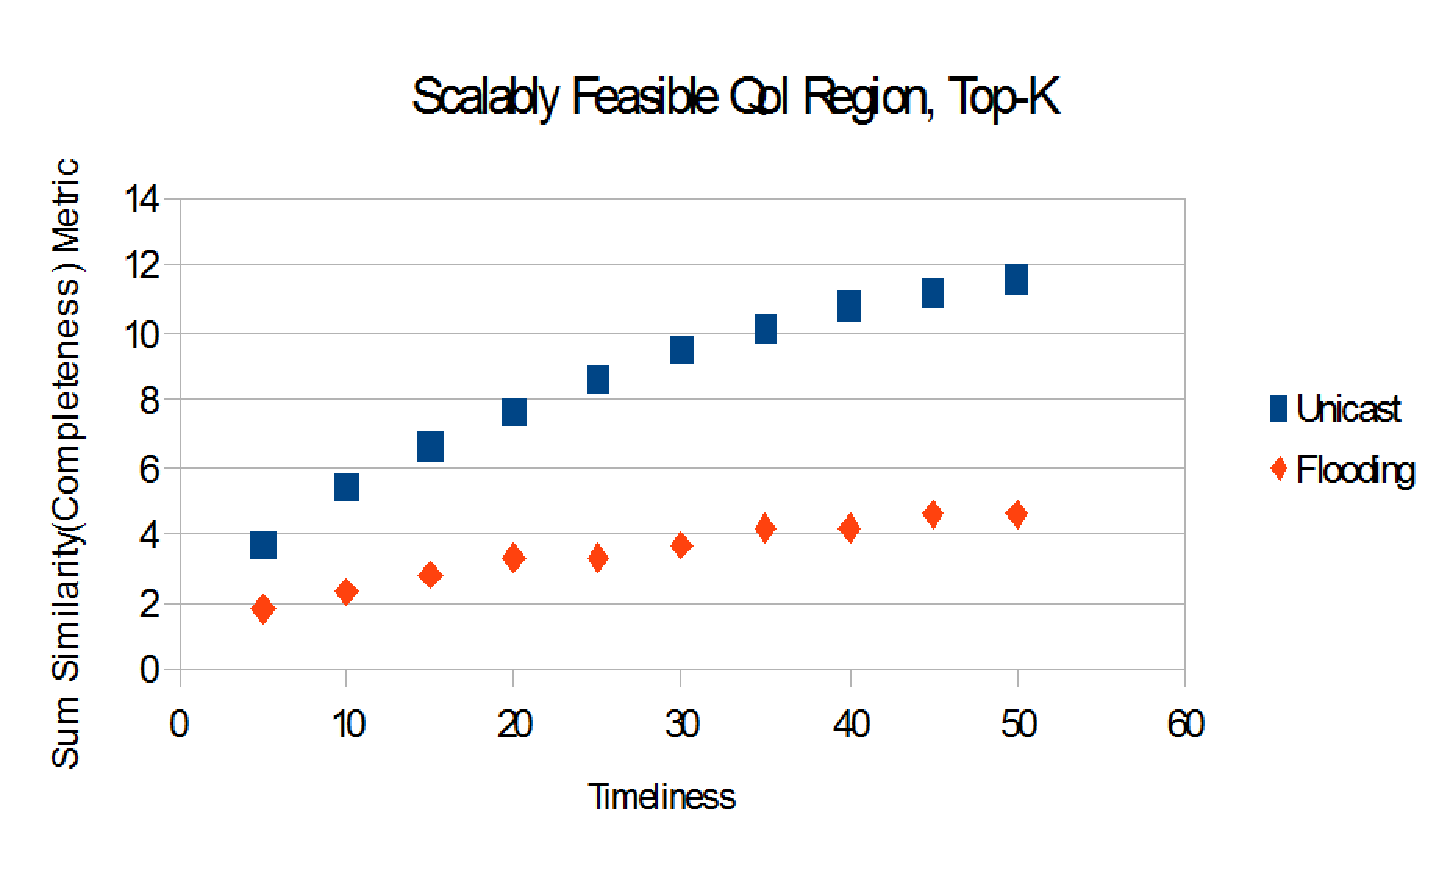
\includegraphics[scale=0.35]{figures/topkScalR.pdf}
    \caption{Feasible Scalability Region of Top-K Algorithm}
    \label{fig:topkScalR}
\end{figure}

\begin{figure}
    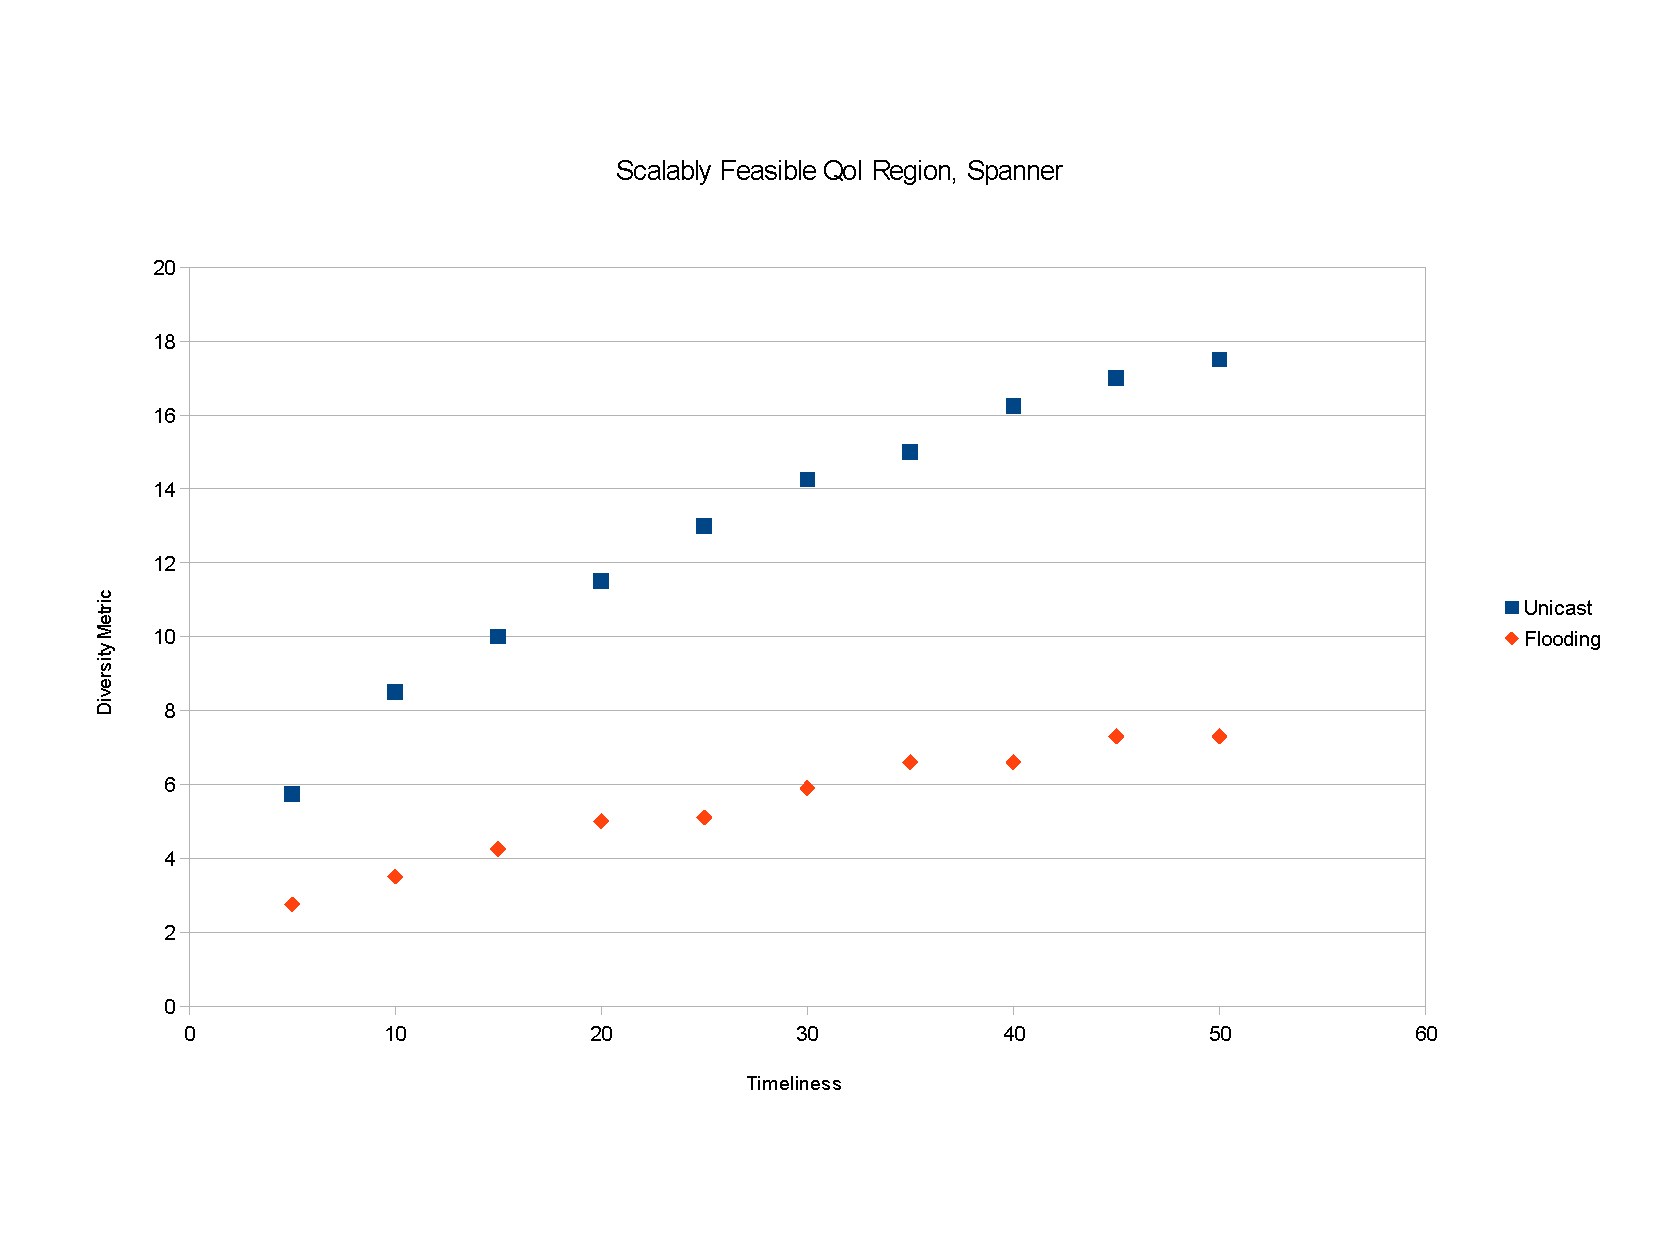
\includegraphics[scale=0.35]{figures/spanScalR.pdf}
    \caption{Feasible Scalability Region of Spanner Algorithm}
    \label{fig:spanScalR}
\end{figure}

As expected, the feasible QoI region is smaller for flooding compared with unicast. Moreover, these regions clearly demonstrate the tradeoff between the completeness/diversity that can be obtained and the timeliness that can be tolerated. 



\section{Conclusion}
\label{sec:conclusion}

Wrap it up with the highlights/takeaways.  Maybe also include future work.


% conference papers do not normally have an appendix


% use section* for acknowledgement
%\section*{Acknowledgment}


%The authors would like to thank...


% trigger a \newpage just before the given reference
% number - used to balance the columns on the last page
% adjust value as needed - may need to be readjusted if
% the document is modified later
%\IEEEtriggeratref{8}
% The "triggered" command can be changed if desired:
%\IEEEtriggercmd{\enlargethispage{-5in}}

% references section

% can use a bibliography generated by BibTeX as a .bbl file
% BibTeX documentation can be easily obtained at:
% http://www.ctan.org/tex-archive/biblio/bibtex/contrib/doc/
% The IEEEtran BibTeX style support page is at:
% http://www.michaelshell.org/tex/ieeetran/bibtex/
%\bibliographystyle{IEEEtran}
% argument is your BibTeX string definitions and bibliography database(s)
%\bibliography{IEEEabrv,../bib/paper}
%
% <OR> manually copy in the resultant .bbl file
% set second argument of \begin to the number of references
% (used to reserve space for the reference number labels box)
%\begin{thebibliography}{1}


\bibliographystyle{unsrt}

\bibliography{references}

%\bibitem{IEEEhowto:kopka}
%H.~Kopka and P.~W. Daly, \emph{A Guide to \LaTeX}, 3rd~ed.\hskip 1em plus
%  0.5em minus 0.4em\relax Harlow, England: Addison-Wesley, 1999.

%\end{thebibliography}




% that's all folks
\end{document}


